\subsection{约化李代数}

定义 4. 若一个李代数的伴随表示是半单的，则称该李代数为约化的。

命题 5. 设 \(\mathfrak{g}\) 是李代数，\(\mathfrak{r}\) 是其根基。以下条件等价：

\begin{enumerate}
\def\labelenumi{(\alph{enumi})}
\item
  g 是约化的。
\item
  \(\mathcal{D}\mathfrak{g}\) 是半单的。
\item
  \(\mathfrak{g}\) 是一个半单代数与一个交换代数的乘积。
\item
  \(\mathfrak{g}\) 有一个有限维表示，使得与之相关的双线性形式非退化。
\item
  \(\mathfrak{g}\) 有一个忠实的有限维半单表示。
\item
  g 的幂零根为零。
\item
  r 是 g 的中心。
\item
  \(\Rightarrow\) (b)：若 \(\mathfrak{g}\) 的伴随表示是半单的，则 \(\mathfrak{g}\) 是极小非零理想 \(a_{i}\) 的直和，因而 \(\mathfrak{g}\) 同构于各 \(a_{i}\) 的乘积；而 \(a_{i}\) 除 \(\{0\}\) 和 \(a_{i}\) 外没有别的理想，所以它或者是单的，或者是一维交换的。因此 \(\mathcal{D}\mathfrak{g}\) 等于那些单的 \(a_{i}\) 的乘积，因而是半单的。
\item
  \(\Rightarrow\) (c)：若 \(\mathcal{D}\mathfrak{g}\) 是半单的，则 \(\mathfrak{g}\) 同构于 \(\mathcal{D}\mathfrak{g}\) 与某个李代数 \(\mathfrak{h}\) 的乘积（第 1 号，命题 1 的推论 1）；\(\mathfrak{h}\) 同构于 \(\mathfrak{g}/\mathcal{D}\mathfrak{g}\)，因而是交换的。
\item
  \(\Rightarrow\) (d)：设 \(g_{1}\) 和 \(g_{2}\) 是两个李代数，\(\rho_{i}\) 是 \(g_{i}\) 的有限维表示，\(\beta_{i}\) 是 \(g_{i}\) 上与 \(\rho_{i}\) 相关的双线性形式（i = 1, 2）；\(\rho_{1}\) 和 \(\rho_{2}\) 可看作 \(g = g_{1} \times g_{2}\) 的表示；令 \(\rho\) 为它们的直和。显然，与 \(\rho\) 相关的 g 上的双线性形式是 \(\beta_{1}\) 与 \(\beta_{2}\) 的直和，因而当 \(\beta_{1}\) 和 \(\beta_{2}\) 非退化时它也是非退化的。为证明 (c) \(\Rightarrow\) (d)，只需考虑以下 2 种情形：(1) g 是半单的；此时伴随表示的相关形式是 Killing 形式，因而非退化；(2) g = K；此时 g 在 K 上的恒等表示有一个非退化的相关双线性形式。
\end{enumerate}

\((d) \Rightarrow (e)\)：令 \(\rho\) 为 \(g\) 的有限维表示，\(\beta\) 为相关双线性形式；根据§4，第 3 号的命题 4，存在 \(\sigma\) 在 \(g\) 上的有限维半单表示，使得 \(n\) 是 \(\sigma\) 的核，且 \(g\) 关于 \(\beta\) 与之正交。若 \(\beta\) 非退化，则 \(n = \{0\}\)，因而 \(\sigma\) 是忠实的。

\begin{enumerate}
\def\labelenumi{(\alph{enumi})}
\setcounter{enumi}{4}
\tightlist
\item
  \(\Rightarrow\) (f)：这是显然的。
\end{enumerate}

\((f) \Rightarrow (g)\)：若 g 的幂零根 \(g\) 为零，则 \(\mathcal{D}g \cap r\) 为零（\(\S 5\)，第 3 号，定理 1）；由于 \([g, r] \subset \mathcal{D}g \cap r\)，\(r\) 是 \(g\) 的中心。

\begin{enumerate}
\def\labelenumi{(\alph{enumi})}
\setcounter{enumi}{6}
\tightlist
\item
  \(\Rightarrow\) (a)：若 \(\mathfrak{r}\) 是 \(\mathfrak{g}\) 的中心，则 \(\mathfrak{g}\) 的伴随表示可视为 \(\mathfrak{g} / \mathfrak{r}\) 的一个表示，而后者是半单李代数（§ 5，第 2 号，命题 3）；因此该表示是半单的（定理 2）。
\end{enumerate}

备注。若李代数 g 能分解为一个交换李代数 a 和一个半单李代数 b 的乘积 \(a \times b\)，则此分解是唯一的。更确切地说，g 的中心等于 a 和 b 的中心的乘积，因而等于 a。而 \(\mathcal{D}g = \mathcal{D}a \times \mathcal{D}b = b\)。

推论。 (a) 每个约化代数的有限乘积都是约化代数。

\begin{enumerate}
\def\labelenumi{(\alph{enumi})}
\setcounter{enumi}{1}
\item
  如果 \(\mathfrak{g}\) 是中心为 \(\mathfrak{c}\) 的约化李代数，则 \(\mathfrak{g}\) 的每个理想都是一个直因子，是它与 \(\mathfrak{c}\) 及 \(\mathcal{D}\mathfrak{g}\) 的交的乘积，并且是约化李代数。
\item
  约化李代数的每个商都是约化李代数。
\end{enumerate}

断言 (a) 例如由命题 5 的条件 (c) 得到。

设 g 是约化的。令 a 为 g 的一个理想。由于 g 的伴随表示是半单的，a 有一个补理想 b，且 g 可与 \(a \times b\) 等同。对所有 \(x \in g\)，令 \(\rho(x)\) 为 \(ad_{g}x\) 在 a 上的限制。于是 \(\rho\) 是 g 的半单表示，在 b 上为零，并且在取商后定义出 a 上的伴随表示。因此 a 是约化的。同样，g/a 和 b（它们同构）都是约化的。最后，令 \(b, b'\) 为 a 和 b 的中心；则 \(a = b \times Da\)、\(b = b' \times Db\)、\(b \times b' = c\)、\(Da \times Db = Dg\)；所以 \(a = (a \cap c) + (a \cap Dg)\)。

命题 6. 设 g 是李代数，r 是其根基，s 是其幂零根。

\begin{enumerate}
\def\labelenumi{(\alph{enumi})}
\item
  \(\mathfrak{s} = [\mathfrak{g},\mathfrak{r}] = \mathcal{D}\mathfrak{g}\cap \mathfrak{r}.\)
\item
  s 是 g 关于与 g 的有限维表示相关的双线性形式的正交补的交。
\end{enumerate}

显然 \([\mathfrak{g},\mathfrak{r}]\subset \mathcal{D}\mathfrak{g}\cap \mathfrak{r}\)。现在 \(\mathcal{D}\mathfrak{g}\cap \mathfrak{r} = \mathfrak{s}\)，由§5，第 3 号的定理 1 得到。令 \(\mathfrak{g}' = \mathfrak{g}/[\mathfrak{g},\mathfrak{r}]\)，令 \(f\) 为从 \(\mathfrak{g}\) 到 \(\mathfrak{g}'\) 上的典范同态；则 \(f(\mathfrak{r})\) 是 \(r'\)，即 \(\mathfrak{g}'\) 的根基（第 2 号，命题 2 的推论 3），因而 \([\mathfrak{g}',\mathfrak{r}'] = \{0\}\)，且 \(r'\) 是 \(\mathfrak{g}'\) 的中心；所以（命题 5）\(\mathfrak{g}'\) 有有限维忠实半单表示，从而 \(\mathfrak{s}\subset [\mathfrak{g},\mathfrak{r}]\)。这就证明了 (a)。

令 \(t\) 为 \(\mathfrak{g}\) 关于与 \(\mathfrak{g}\) 的有限维表示相关的双线性形式的正交补之交。则 \(\mathfrak{s} \subset t\)（\(\S 4\)，第 3 号，命题 4 (d)）。另一方面，\(\mathfrak{g}/\mathfrak{s}\) 有一个有限维忠实半单表示，因而（命题 5）有一个有限维表示 \(\rho\)，使得与之相关的双线性形式非退化；将它视为 \(\mathfrak{g}\) 的表示，\(\rho\) 有一个相关双线性形式 \(\beta\) 在 \(\mathfrak{g}\) 上，而 \(\mathfrak{g}\) 关于 \(\beta\) 的正交补是 \(\mathfrak{s}\)，从而 \(t \subset \mathfrak{s}\)。因此 \(t = \mathfrak{s}\)。

\pandocbounded{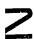
\includegraphics[keepaspectratio]{images/part001_ead1ec0a.jpg}}

即使 \(s \neq \{0\}\)，g 上也可能存在非退化对称双线性形式（习题 18 (c)）。当然，这样的形式并不与 g 的任何表示相关。

推论。设 \(\mathfrak{g},\mathfrak{g}'\) 是李代数，\(\mathfrak{s}\)（分别为 \(\mathfrak{s}'\)）是 \(\mathfrak{g}\)（分别为 \(\mathfrak{g}'\)）的幂零根，\(f\) 是从 \(\mathfrak{g}\) 到 \(\mathfrak{g}'\) 上的一个同态。

\begin{enumerate}
\def\labelenumi{(\alph{enumi})}
\item
  则 \(\mathfrak{s}' = f(\mathfrak{s})\)。
\item
  \(\mathfrak{g}'\) 是约化的，当且仅当 \(f\) 的核包含 \(\mathfrak{s}\)。
\end{enumerate}

若 \(\mathfrak{r},\mathfrak{r}'\) 是 \(\mathfrak{g},\mathfrak{g}',\) 的根基，则 \(\mathfrak{s}' = [\mathfrak{g}',\mathfrak{r}'] = [f(\mathfrak{g}),f(\mathfrak{r})] = f([ \mathfrak{g},\mathfrak{r}]) = f(\mathfrak{s})\)。断言 (b) 是 (a) 的直接推论。

